\chapter[Pruebas]{Pruebas}
\label{cp:testing}

\parindent0pt

El presente capítulo aborda el proceso de pruebas del prototipo, un componente central del Modelo en V de ingeniería de software que rige el desarrollo de este trabajo. Este proceso de validación, que abarca la totalidad de la segunda mitad del modelo, tiene como objetivo principal verificar que el prototipo se alinee con los requerimientos y el diseño definidos en las fases previas. El proceso de pruebas se estructura en un ciclo progresivo, donde la granularidad de la validación disminuye a medida que se avanza en las etapas, comenzando por las unidades de código más pequeñas y atómicas (pruebas unitarias), avanzando con pruebas de integración entre los módulos del sistema, hasta alcanzar la validación del sistema en su totalidad (pruebas de sistema y de aceptación). La naturaleza de estas pruebas varía entre automatizada y manual. Las pruebas automatizadas, si bien requieren una inversión inicial, se ejecutan de manera instantánea y repetible, lo cual resulta ideal para verificar comportamientos de forma constante. Por su parte, las pruebas manuales, aunque resultan más lentas de ejecutar, permiten una validación completa de los flujos de usuario y la experiencia general del sistema.

A continuación, se detallan las cuatro etapas de pruebas integrales realizadas en el proyecto:

\begin{itemize}
\item Pruebas Unitarias: se enfocan en la validación del código a nivel de componente.
\item Pruebas de Integración: verifican la interacción entre los módulos del sistema.
\item Pruebas de Sistema: validan el cumplimiento de los requerimientos funcionales y no funcionales del prototipo en su totalidad.
\item Pruebas de Aceptación con Usuarios: validan que el prototipo cumpla con las expectativas y necesidades del usuario final.
\end{itemize}
La Tabla \ref{tab:testing-comparison} presenta una comparación de estas etapas, destacando sus características y su alcance, como una guía visual para comprender la metodología de prueba aplicada.

\begin{table}[!htpb]
\centering
\caption{Comparación de las etapas de prueba del prototipo de trazabilidad de vidrio}
\label{tab:testing-comparison}
\begin{tabular}{|l|l|l|l|l|}
\hline
\textbf{Etapa de Prueba} & \textbf{Frecuencia de Ejecución} & \textbf{Tipo} & \textbf{Complejidad} & \textbf{Alcance} \
\hline
Pruebas Unitarias & Continua (por cada cambio) & Automatizada & Baja & Componentes \
Pruebas de Integración & Antes de cada despliegue & Automatizada & Media & Interacción de componentes \
Pruebas de Sistema & Al finalizar la implementación & Manual & Media-Alta & Requerimientos funcionales \
Pruebas de Aceptación & Al finalizar la implementación & Manual & Alta & Experiencia del usuario \
\hline
\end{tabular}
\end{table}

A lo largo de este capítulo, se detallará la gestión de las incidencias halladas durante las pruebas. Los errores detectados en cada etapa de prueba fueron registrados y se les dio seguimiento en la herramienta Jira, asegurando que cada problema se resolviera antes de avanzar a la siguiente fase. El Apéndice \ref{cp:tests-execution-results} contiene los detalles de la ejecución de cada prueba, los resultados obtenidos y la gestión de las incidencias documentadas. A continuación, se describen en detalle cada una de las etapas de prueba mencionadas, proporcionando una visión completa del proceso de validación del prototipo.

\section{Pruebas Unitarias}
\label{sec:unit-testing}

Las pruebas unitarias constituyen la base de la pirámide de pruebas y se corresponden directamente con la fase de codificación del Modelo en V. Su objetivo es validar la unidad más pequeña de código, como una función o un método, de forma aislada del resto del sistema. La naturaleza atómica de estas pruebas permite verificar que cada componente individual se comporte de acuerdo con las especificaciones de diseño antes de ser integrado con otras partes del prototipo. Para este proyecto, se implementaron pruebas unitarias automatizadas para permitir una verificación continua de la integridad del código a lo largo de todo el proceso de implementación y luego de cada modificación de código posterior.

El desarrollo de cada módulo del prototipo se realizó de forma conjunta con la escritura de sus pruebas unitarias. Se utilizó el framework Jest \footnote{https://jestjs.io/} en las tres capas del proyecto (contratos inteligentes, API y frontend), aunque con configuraciones específicas para cada entorno. Por ejemplo, en los contratos inteligentes, las pruebas unitarias se orientaron a verificar que la lógica de negocio se ejecute correctamente y que el estado de los contratos cambie como se espera. En el backend, se enfocaron en validar la lógica de negocios. En el frontend, se validó el comportamiento de los componentes, su estado interno y la interacción con la API.

Un indicador representativo de la calidad del testing unitario es la covertura de código (conocida comunmente como \textit{coverage}), que mide el porcentaje de código fuente ejecutado por las pruebas. Este valor, si bien no garantiza la ausencia de errores, es una herramienta útil para evaluar la robustez del código. Los requisitos de cobertura mínima se definieron en función de la criticidad de cada módulo del sistema: 

\begin{itemize}
\item Contratos Inteligentes: se requirió una cobertura mínima del 100\%. Dado que los contratos son la base del sistema de trazabilidad y no pueden modificarse una vez desplegados, resulta fundamental garantizar que todos los caminos de ejecución del código estén cubiertos para minimizar el riesgo de errores una vez desplegados. Este es un estándar de la industria para contratos inteligentes.
\item API Backend: se requirió una cobertura mínima del 80\%. Dado que la API representa el componente central del sistema como responsable de la comunicación con la blockchain y la base de datos, resulta relevante garantizar la calidad del código y minimizar el riesgo de errores en el manejo de datos. Por este motivo, se ha elegido este umbral de cobertura, que es un estándar habitual en la industria para aplicaciones de propósito general.
\item Aplicación Frontend: se estableció una cobertura mínima del 60\%. Dado que el frontend del prototipo tiene fines demostrativos y no es una parte crítica del sistema, este umbral se consideró suficiente para garantizar el correcto funcionamiento de la interfaz de usuario sin requerir un esfuerzo excesivo en la escritura de pruebas.
\end{itemize}

El proceso de pruebas unitarias permitió identificar y corregir algunos errores de manera temprana. Los erorres detectados en esta etapa fueron resueltos de manera inmediata, ya que las pruebas unitarias son cercanas a la implementación y permiten una rápida retroalimentación sobre el estado del código. En la Tabla \ref{tab:unit-testing-summary} se muestra un resumen de las pruebas unitarias realizadas, mientras que en el Apéndice \ref{cp:tests-execution-results} se puede consultar en mayor detalle el listado de casos de prueba.

\begin{table}[!htpb]
\centering
\caption{Resumen de Pruebas Unitarias}
\label{tab:unit-testing-summary}
\begin{tabular}{|l|c|c|c|}
\hline
\textbf{Módulo} & \textbf{Coverage Objetivo} & \textbf{Coverage Alcanzado} & \textbf{Cant. de Pruebas} \
\hline
Contratos Inteligentes & 100\% & 100\% & 98 \
API Backend & 80\% & 90.84\% & 317 \
Aplicación Frontend & 60\% & 65.27\% & 286 \
\hline
\end{tabular}
\end{table}

La ejecución automatizada de las pruebas unitarias proporciona una capa de seguridad que facilita la revalidación del comportamiento del sistema, lo cual es relevante en un prototipo que podría expandirse en un futuro. La validación constante de la base de código antes de cualquier despliegue favorece la estabilidad y la calidad del sistema a largo plazo. Una vez que se ha verificado el funcionamiento de cada componente del sistema de forma individual, es posible continuar con la siguiente etapa de validación, donde se verificará la correcta interacción entre los módulos del sistema.

\section{Pruebas de Integración}
\label{sec:integration-testing}

Las pruebas de integración se sitúan en la siguiente capa de la pirámide de pruebas. Su objetivo principal consiste en verificar que los distintos componentes y módulos del sistema interactúen entre sí de manera correcta y consistente. A diferencia de las pruebas unitarias, que validan el funcionamiento aislado de una unidad de código, las pruebas de integración evalúan el flujo de datos y las interacciones entre componentes para asegurar que sus interfaces y responsabilidades estén debidamente sincronizadas. Esta etapa de prueba se corresponde con la fase de diseño de componentes del Modelo en V, donde se definen las interacciones entre los módulos del sistema.

Para este proyecto, las pruebas de integración se diseñaron para ser automatizadas y se enfocaron en los puntos de interacción más críticos del sistema. El entorno de prueba se configuró para simular un escenario lo más cercano posible a un entorno real, pero aislado, sin hacer uso de funcionalidades simuladas. Por ejemplo, mientras que durante las pruebas unitarias se simularon los datos que debería retornar la blockchain para probar la funcionalidad de la API, durante las pruebas de integración se utilizaron datos reales obtenidos de un entorno virtual de la red blockchain. De esta manera, se pudo validar que la comunicación entre los módulos funciona correctamente en un contexto más realista.

El proceso de pruebas de integración no detectó fallos en la interacción entre los módulos. Se realizaron pruebas de integración para 18 casos de uso del sistema, los cuales se han documentado en el Apéndice \ref{cp:tests-execution-results}. La ejecución de estas pruebas proporciona una capa de verificación adicional del sistema y se recomienda ejecutarlas de forma rutinaria antes de cada despliegue en un entorno productivo para mitigar los riesgos asociados a los cambios en el código que puedan afectar la interacción entre los módulos del sistema. Una vez que se ha validado la interacción de los componentes, la siguiente etapa consiste en verificar que el sistema en su totalidad cumpla con los requisitos funcionales y no funcionales definidos al comenzar el proyecto.

\section{Pruebas de Sistema}
\label{sec:system-testing}

Las pruebas de sistema constituyen la siguiente fase en el ciclo de validación, y tienen como propósito verificar que el prototipo, en su conjunto, cumple con los requerimientos funcionales y no funcionales definidos al comenzar el proyecto. Esta etapa se corresponde con el diseño de arquitectura en el Modelo en V, y su objetivo es evaluar el comportamiento del sistema de manera integral para asegurar que la arquitectura implementada efectivamente logra cumplir los requisitos establecidos.

A diferencia de las pruebas unitarias y de integración, que fueron automatizadas, las pruebas de sistema se ejecutaron de manera manual. En primer lugar, se documentó de forma detallada cada caso de prueba a ejecutarse, incluyendo un título, requerimientos asociados, los pasos a seguir desde la perspectiva de un usuario, los datos de entrada (en caso de requerirlos) y los resultados esperados. Posteriormente, se ejecutó de forma manual cada caso de prueba, siguiendo los pasos definidos y registrando los resultados obtenidos. La metodología consistió en interactuar con la interfaz de usuario (frontend) del sistema y seguir los pasos detallados en el caso. En estas pruebas, se utilizó el sistema completo desplegado en el entorno de pruebas, sin emplear datos simulados ni probar funcionalidades de forma aislada. Esto permitió una validación precisa del comportamiento del prototipo, desde la perspectiva de un usuario, en un entorno que replicaba la realidad.

A su vez, también se incluyeron pruebas de requerimientos no funcionales en esta etapa, como son la escalabilidad, el rendimiento y la seguridad del sistema. A pesar de las limitaciones de recursos del entorno de pruebas (debido a que se utilizaron plataformas gratuitas), se llevaron a cabo pruebas controladas para validar que el sistema puede cumplir con estos requerimientos en un entorno real. Los detalles y resultados de estas pruebas se documentaron junto con los casos de prueba funcionales en el Apéndice \ref{cp:tests-execution-results}.

El proceso de pruebas de sistema incluyó un total de 55 casos de prueba y resultó en la identificación de 7 incidencias, las cuales fueron registradas y rastreadas en la herramienta Jira hasta su resolución. La ejecución de estas pruebas permitió identificar y corregir errores, pero también puede servir como una base para futuras pruebas de regresión del sistema, ayudando a prevenir que cualquier cambio o nueva funcionalidad no afecte negativamente el comportamiento actual. Luego de esta etapa, el prototipo ya está listo para ser presentado a un grupo reducido de usuarios, quienes serán responsables de evaluar su funcionalidad durante las pruebas de aceptación.

\section{Pruebas de Aceptación con Usuarios}
\label{sec:user-acceptance-testing}

La fase final de validación del prototipo corresponde a las Pruebas de Aceptación con Usuarios (\textit{UAT}, por sus siglas en inglés). Esta etapa se enfoca en verificar que el sistema no solo funcione correctamente a nivel técnico, sino que también satisfaga las necesidades y expectativas del usuario final, tal como se definieron en la etapa de modelado de requerimientos del Modelo en V. En esta instancia, un grupo reducido de usuarios es convocado para utilizar el sistema en un entorno controlado, de forma similar a cómo utilizaría el sistema en su rutina habitual. 

Dada la naturaleza de este trabajo como proyecto académico, la obtención de usuarios reales de la industria del vidrio para la ejecución de estas pruebas presentó una limitación. No obstante, se llevó a cabo un experimento controlado con un grupo de usuarios voluntarios del entorno académico. El experimento se realizó en un laboratorio de computación, donde cada usuario voluntario contó con una computadora de escritorio con acceso a Internet, desde donde pudo acceder al frontend del prototipo desplegado en el entorno de pruebas. La metodología de la prueba combinó una fase guiada y una fase libre, creando un entorno mixto, donde los participantes recibieron una guía para ejecutar una serie de casos de prueba predefinidos, seguidos de un período de exploración libre del sistema. Este enfoque permitió validar tanto los flujos de trabajo específicos como la usabilidad general del prototipo. Los participantes evaluaron tanto los requerimientos funcionales (por ejemplo, la capacidad de registrar un lote de vidrio) como los no funcionales (como la facilidad de uso y la transparencia de la información) registrando en una planilla la descripción del caso de prueba ejecutado y el resultado obtenido.

La ejecución de las pruebas generó una retroalimentación detallada que se utilizó para identificar y resolver fallos, así como para mejorar la experiencia de usuario (UX) y el diseño de la interfaz. Se registraron en Jira un total de 9 incidencias y 3 sugerencias recibidas para su posterior seguimiento. Como resultado directo de estas pruebas, se realizaron mejoras en los flujos de navegación, la presentación de los datos de trazabilidad y el diseño visual de la aplicación. En el Apéndice \ref{cp:tests-execution-results} encuentran documentados los casos de prueba ejecutados durante el experimento y la retroalimentación de los participantes. En las Figuras \ref{fig:uat-picture-1} y \ref{fig:uat-picture-2} se pueden observar fotografías tomadas durante la ejecución del experimento, donde se puede observar a los usuarios voluntarios del experimento utilizando el prototipo.

\begin{figure}[!htb]
\centering
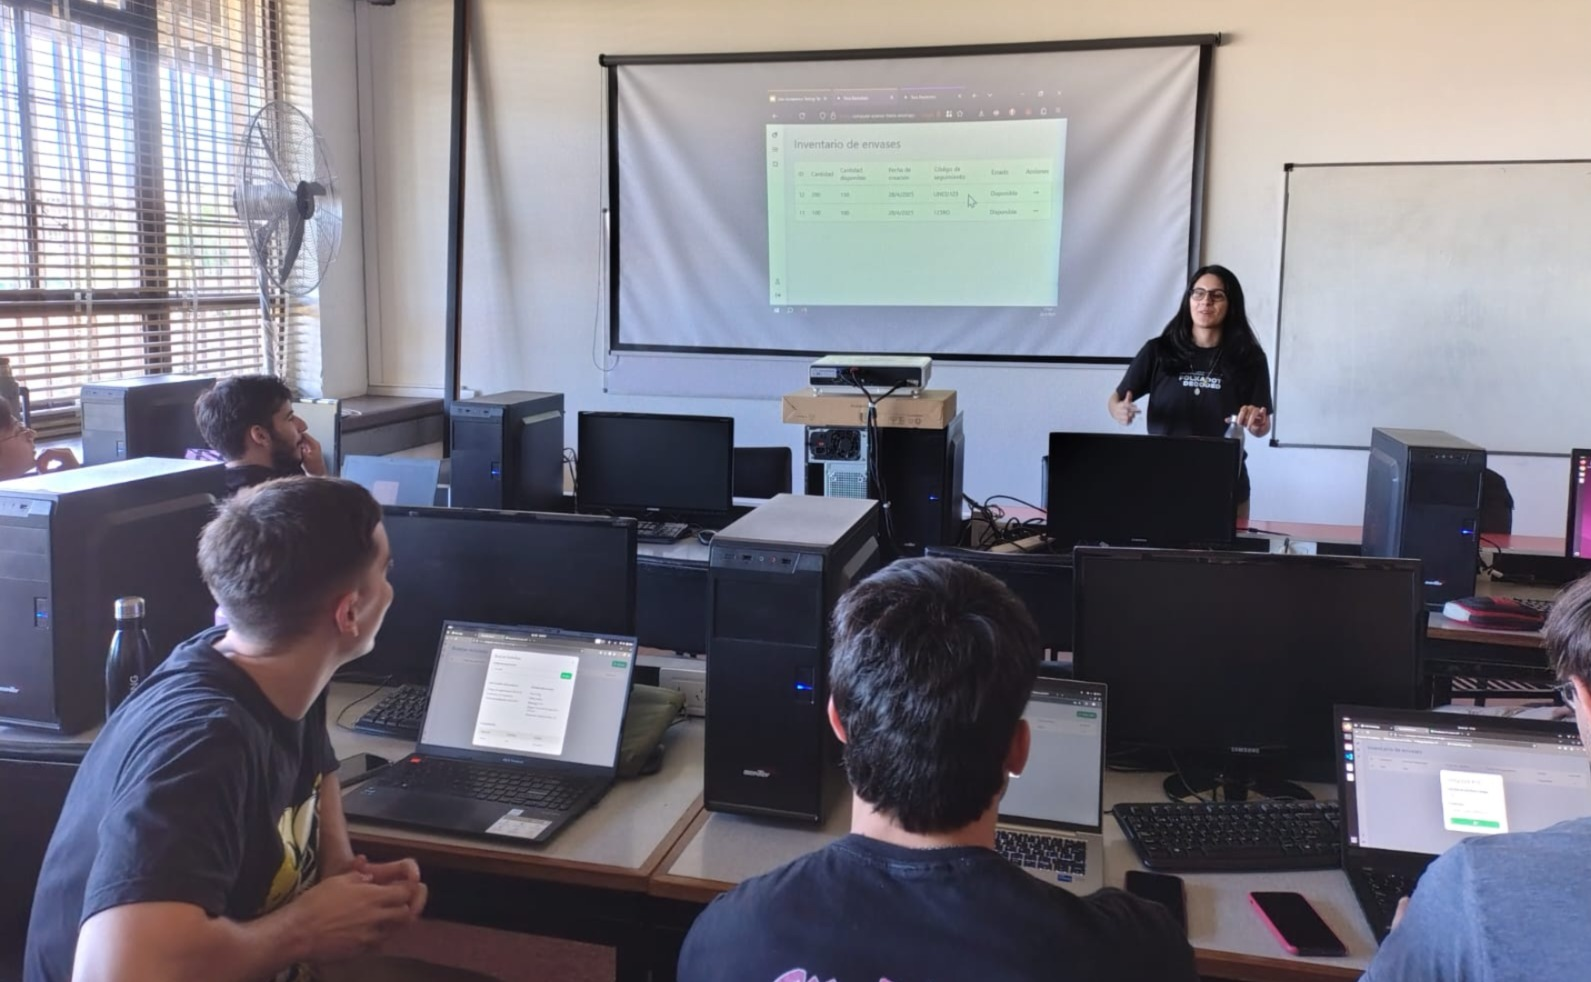
\includegraphics[width=0.8\textwidth]{Figures/uat-1.jpg}
\caption{Usuarios interactuando con el prototipo durante prueba guiada}
\label{fig:uat-picture-1}
\end{figure}

\begin{figure}[!htb]
\centering
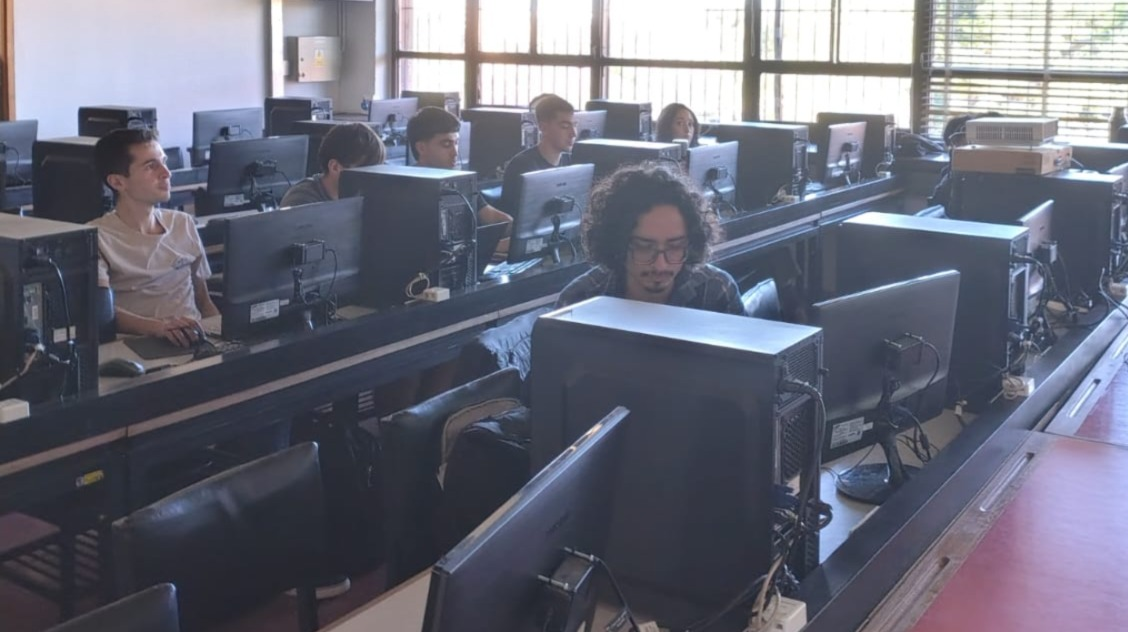
\includegraphics[width=0.8\textwidth]{Figures/uat-2.jpg}
\caption{Usuarios voluntarios durante el experimento}
\label{fig:uat-picture-2}
\end{figure}

Al finalizar la etapa de pruebas con usuarios, se llevó a cabo una revisión de los resultados obtenidos. El riguroso proceso de pruebas llevado a cabo, desde las unidades más pequeñas de código hasta la validación con usuarios voluntarios, demostró que el prototipo desarrollado es funcional y está alineado con los requerimientos originales del proyecto. Esta etapa de validación confirma la viabilidad del sistema de trazabilidad del vidrio basado en blockchain, estableciendo un precedente sólido para su potencial escalabilidad y aplicación en un entorno productivo. La finalización de esta fase marca la conclusión del ciclo de vida del desarrollo del software de este proyecto académico, cuyos principales hallazgos, lecciones aprendidas y oportunidades de mejora se resumen en el siguiente capítulo.
